\chapter{Ontwerp van het project}
\label{hoofdstuk:ontwerp}

Eenmaal de belangrijkste vereisten gekend zijn kan er een ontwerp opgetekend worden. Daarom even de grote lijnen die te concluderen vallen uit hoofdstuk \ref{hoofdstuk:doelen}:

\begin{itemize}
  \item De data en het visuele aspect van de applicatie moeten zo ontkoppeld mogelijk zijn, elk moet apart uitbreidbaar zijn
  \item Zeer grote hoeveelheden data moeten vlot kunnen behandeld en genavigeerd worden: zoeken, filteren, sorteren, aanpassen, \ldots
  \item De data moet zowel centraal als decentraal toegankelijk zijn en synchronisatie toestaan
  \item Compatibiliteit met de reeds geschreven onderdelen van het project moet indien mogelijk bewaard blijven
  \item Om het ontwerp te verifi\"eren moet een werkend programma gemaakt worden, gebruiksvriendelijkheid, functionaliteit en snelheid zijn hierbij belangrijk
\end{itemize}

\section{De grote lijnen}
Van alle vereisten die rechtstreeks invloed kunnen uitoefenen op de architectuur, is de splitsing van de data en de visualisatie waarschijnlijk de meest fundamentele. Een beproefde aanpak om dit te realizeren is het ontwerppatroon genaamd \emph{Model-View-Controller (MVC)}\footnote{Een algemeen overzicht kan men bijvoorbeeld bekomen op \url{http://en.wikipedia.org/wiki/Model-view-controller}}.\\

Het doel is een ontwerp te maken waarin we een visualisatiemethode kunnen verbinden aan de juiste databron. Enkele zaken moeten echter nog vastgelegd worden, namelijk: wat is de basiseenheid van data? Waar zal een visualisatiemodule achter vragen? Zoals in figuur~\ref{fig:flow} te zien is, ligt de focus bij dit project op koppelingen van fragmenten in plaats van fragmenten op zich. Er zijn op het eerste zicht twee alternatieven om dit te modelleren. Een eerste mogelijkheid is een soort van \emph{MatchedFragment} die een fragment beschrijft plus een lijst met alle fragmenten die er potentieel aan gekoppeld kunnen worden en op welke locatie. De tweede mogelijkheid is om elk paar een apart object te laten voorstellen (bvb. genaamd \emph{FragmentPair}). Het eerste alternatief lijkt het programmatische voordeel te hebben dat het gemakkelijk is om na te kijken of een fragment reeds ``bezet'' is. Ook zou het dan mogelijk zijn om bijvoorbeeld een grafe op te stellen door van brokstuk naar brokstuk te springen. Echter, dit soort opstelling bevat veel redundantie, een fragment zal op die manier een verwijzing met attributen naar een fragment bevatten, en dit fragment zal op zijn beurt een identieke omgekeerde verbinding hebben. De redundantie vermijden en een verwijzing als een apart object voorstellen waar beide fragmenten naar kunnen verwijzen is eigenlijk niets anders dan de tweede optie (een \emph{FragmentPair}). Daarbij kan het probleem van hoe de ``bezetting'' van een object te weten te komen (alsook de grafe, zoals later zal aangetoond worden) opgelost worden door de vereiste zoekfunctionaliteit van het datamodel te benutten.\\

Eenmaal deze basiseenheid van informatie gekozen, valt de kern van de applicatie volgens MVC uit te beelden als in figuur~\ref{fig:basicprogramflow}.

\begin{figure}[ht]
	\begin{center}
		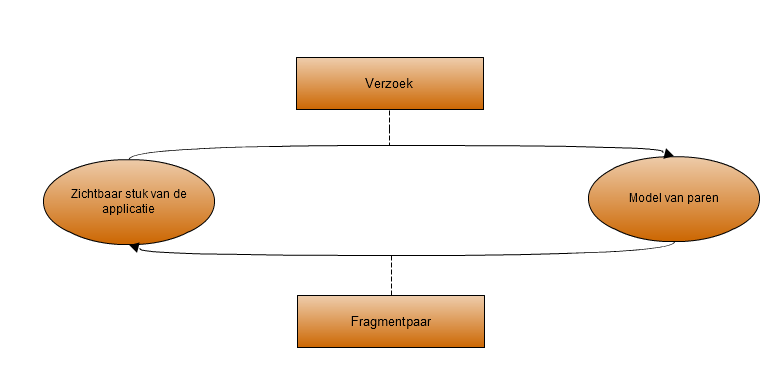
\includegraphics[width=1.0\columnwidth]{images/BasicExecutionFlow.png}
		\caption{Het abstracte model van de applicatie, links staat de \emph{View/Controller} en rechts het \emph{Model}. De controller stuurt een verzoek naar het model voor een bepaalde (sub)set van de data --- al dan niet gesorteerd --- en het model antwoord met alle paren die voldoen aan de criteria}
		\label{fig:basicprogramflow}
	\end{center}
\end{figure}

\section{Modulariteit}
Om het geheel uitbreidbaar te maken is een pluginsysteem gemaakt. Er is een hoofdapplicatie (codenaam ``Tangerine'') die de connectie maakt met de databeheerlaag en verschillende visualisatieplugins kan laden. Het basissysteem zonder modules bestaat uit een manier om een fragmenten en paren-database in te laden en te kiezen welke module op te starten.\\

De eerste en meest uitgewerkte daarvan werd \emph{MatchTileView} gedoopt. Het geeft de paren op dezelfde manier weer als het Browsematches prototype, maar is natuurlijk uitgebreid qua mogelijkheiden. De bespreking van de nieuwe functionaliteiten komt aan het bod in het hoofdstuk over modules.\\

\begin{figure}[ht]
	\begin{center}
		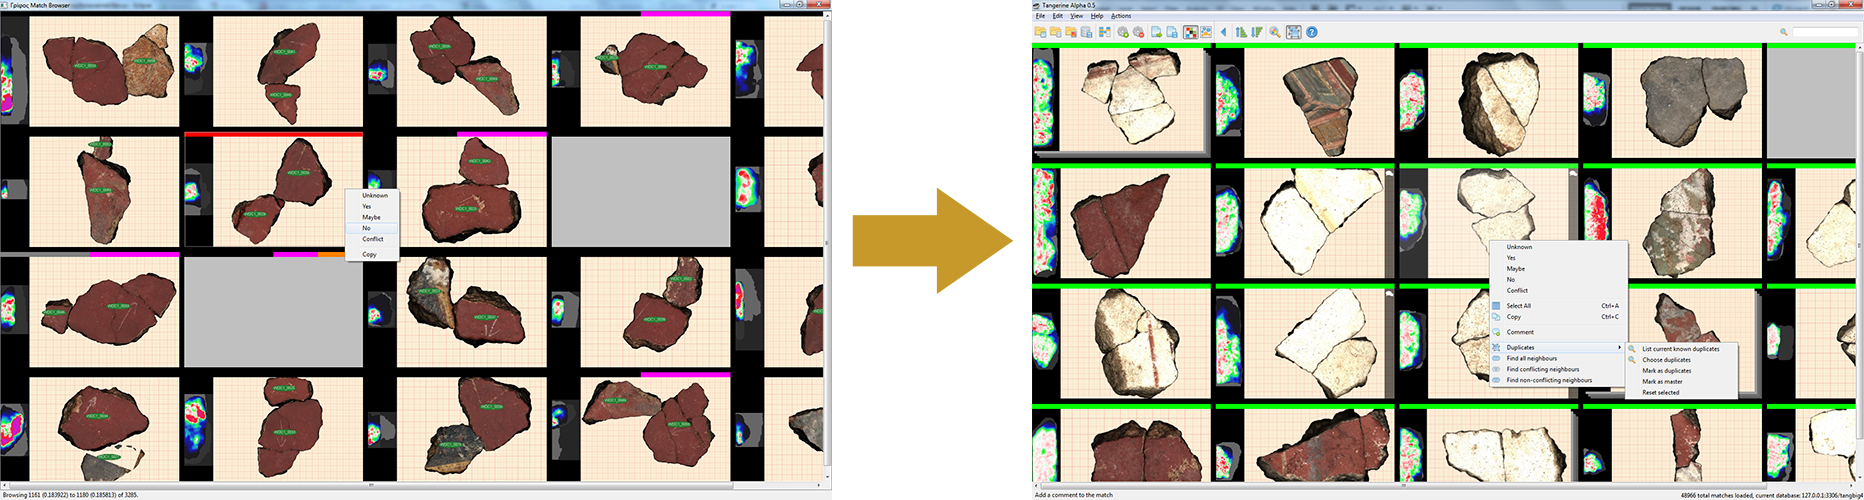
\includegraphics[width=1.0\columnwidth]{images/browsematches-to-tangerine-01.png}
		\caption{De manier van weergeven uit Browsematches werd gekopi\"eerd naar het nieuwe platform, met uitbreidingen}
		\label{fig:browsematchestotang}
	\end{center}
\end{figure}

Elke module krijgt van de applicatie een model toegewezen, dit kan een blanco model zijn zonder criteria of een gedeeld model. Een gedeeld model betekent bijvoorbeeld dat als er een een module beslist om te sorteren op een attribuut zoals ``het verschil van de dikte tussen twee fragmenten'', alle modules die gebruikmaken van ditzelfde model opeens over een gesorteerde dataset beschikken. Via speciale signalen worden zij hiervan op de hoogte gebracht, zodat ze kunnen beslissen of het nodig is een actie te ondernemen. Dit kan handig zijn voor pure visualizatieplugins die geen zoekmogelijkheden aan de gebruiker blootstellen, het kan dan vertrouwen op andere modules om data aan te leveren.\\

Indirecte communicatie via het model is (voorlopig) de enige manier waarop modules elkaar kunnen be\"invloeden. De structuur van de componenten ziet er uit als in figuur~\ref{fig:visualizationlayer}. Merk op dat er een plugin is (\emph{DetailView}) die geen gebruik maakt van fragmentparen maar eerder van een virtueel tafelblad net als Griphos. Zoals eerder aangehaald kunnen fragmentparen automatisch op een tafelblad gezet worden. Dit tafelblad kan dan in 3D weergegeven worden door \emph{DetailView}, waarover later meer.

\begin{figure}[h]
	\begin{center}
		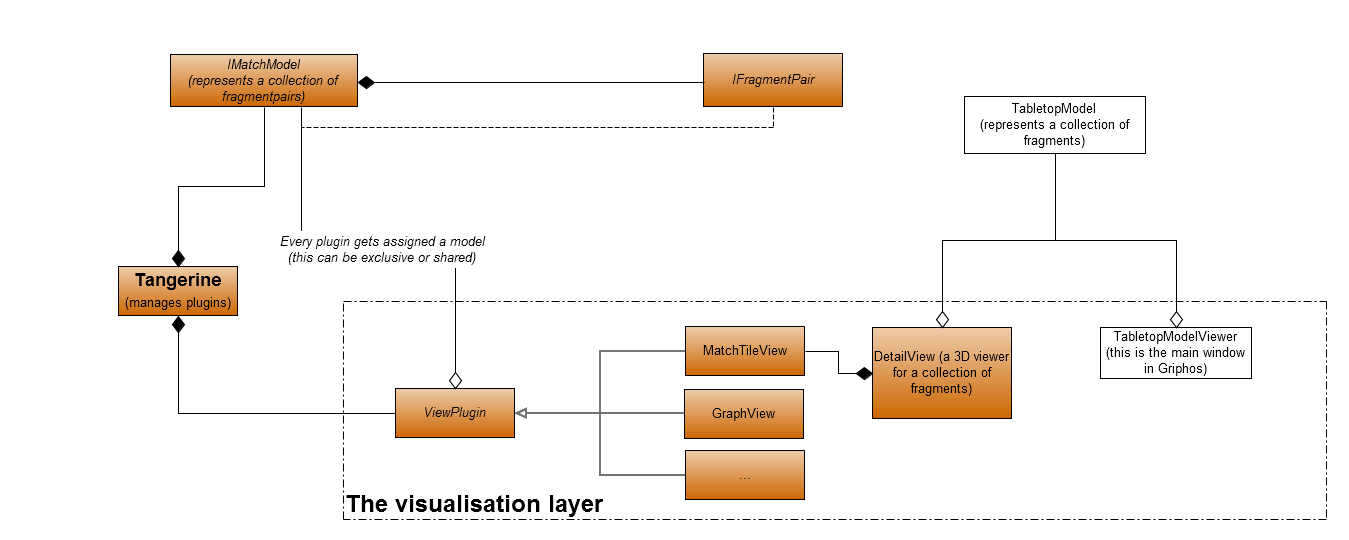
\includegraphics[width=1.0\columnwidth]{images/VisualizationExtract.png}
		\caption{Een vereenvoudigde kijk op de componenten van de visualisatielaag, het hoofdscherm en het model. De componenten in het wit behoren tot de rest van het thera project en zijn niet gemaakt als deel van dit thesisproject.}
		\label{fig:visualizationlayer}
	\end{center}
\end{figure}

\section{De eenheid van informatie: het fragmentenpaar}

Speciale eigenschappen, write-through, \ldots

% DATA
\section{Het beheer van de data}

Redenering: Alles vloeit voort uit de paren, het is voorspelbaar (simpel voor te stellen) en ondubbelzinnig

Het zelf kunnen maken van paren is van secundair belang (volgens de thesis), zij kunnen door de HumanMatcher ingevoerd worden in de grote database

Griphos is zeer nuttig -> identificatie locatie van fragmenten in de bak, etc. -> Tangerine is het ontbrekende middendeel!

Dit betekent echter niet dat beide perspectieven elkaar uitsluiten, integendeeel.
 
[TODO: verhuizen naar ontwerp van database]

\subsection{Het oude systeem: XML-bestanden}

E\'en van de belangrijkste stappen op weg naar een collaboratieve applicatie, is het omvormen van\\

Het ontwerp van het database model en de implementatie details zijn groot genoeg om hun eigen hoofdstuk te verdienen, zij worden later in hoofdstuk [...] besproken.\\

\subsection{Ontleding van de data}
...relationeel van aard => SQL database

\subsubsection{Paren}

\subsubsection{Attributen van paren}

\subsubsection{Complexe informatie die niet in een simpel attribuut past}

\subsection{De vereisten van een database ontwerp}
Zoals in sectie [doelen] omschreven moet de applicatie in staat zijn om data op een uitbreidbare manier uit te lezen en te veranderen, liefst zonder 

\subsection{Complexe informatie voorstellen als een attribuut}
Meta-attributen, VIEWs

\subsection{Verschillende iteraties}

\subsection{Databases samenstellen}

\subsubsection{Geschiedenis bijhouden}

% VISUALISATIE
\section{Visualisatie, een manier om met de data te werken}

\subsection{Model-View-Controller}

\subsection{UML diagramma}

[maak UML diagramma]\\

\subsection{GUI}
Met behulp van de Qt toolkit [link]...

Multi-threading voor responsiviteit

\section{Integratie in thera project}
Gebruik van bibliotheken, ...
Extensie door refactoring: FragmentConf -> IFragmentConf ==> SQLFragmentConf | FragmentConf
Hierdoor is het nodig om de reeds bestaande code van het thera project om te zetten naar het gebruik van IFragmentConf waar mogelijk maar het aanmaken van FragmentConf anderzijds
of FragmentConf ==> SQLFragmentConf
Alternatieve oplossing, geen veranderingen in thera code maar SQLFragmentConf sleept dan veel onnodige ballast mee van FragmentConf

\section{Uitbreidbaarheid}
[afbeeldingen invoegen]\\


[afbeelding invoegen, selectie naar grafe transit!]\\